\chapter{Appendix}
\label{chap:appendix}

Additional material for explanations and results can be found here. There is also a section of parameters and methods that were tried but did not yield positive results. This is done such that other scientist that want to research this or related problems do not need to waste time. 

\section{Negative Results}
\label{sec:stuff_that_did_not_work}

\begin{enumerate}
	\item Given that the aspect ratio of the images from the KITTI dataset are 3:1 we set up an SSD with input size 1000x300 and adapted the feature sizes accordingly. However, the results were comparable to or worse than the 300x300 version but took longer to compute and was therefore discarded.
	\item The values called s\_sizes in the hyperparameters Subsection \ref{subsec:hyperparameters} are calculated according to a minimum value of 0.2 and maximum value of 0.9 with a linear interpolation in between. We changed these values to 0.1 and 0.95 and other combinations. Non of them were more successful than the default ones.
\end{enumerate}

\section{Explanations of the Scattering Transform}

Figure \ref{fig:example2_coefficients} shows a translated version of the image found in section \ref{subsec:scattering_networks}. \\
Figure \ref{fig:example1e_coefficients} shows the scattering coefficients of another object, in this case an ellipse, to see the properties of rounded edges. \\
Figure \ref{fig:example2e_coefficients} shows a scaled version of \ref{fig:example1e_coefficients}. 

%translated example1 = example2
\begin{figure}
	\centering
	\begin{tabular}{cc}
		\subfloat[]{\fbox{
\includegraphics[width=4.5cm]{images/0000011_03.jpg}}} 
		& \subfloat[]{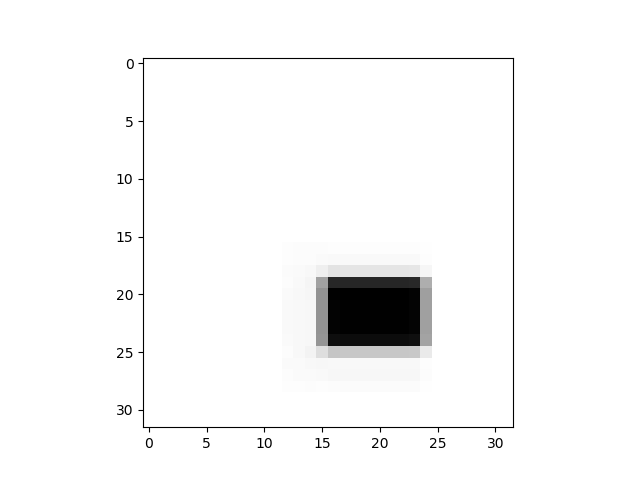
\includegraphics[width=7cm]{images/example2_0ord.png}}\\
		
		\subfloat[]{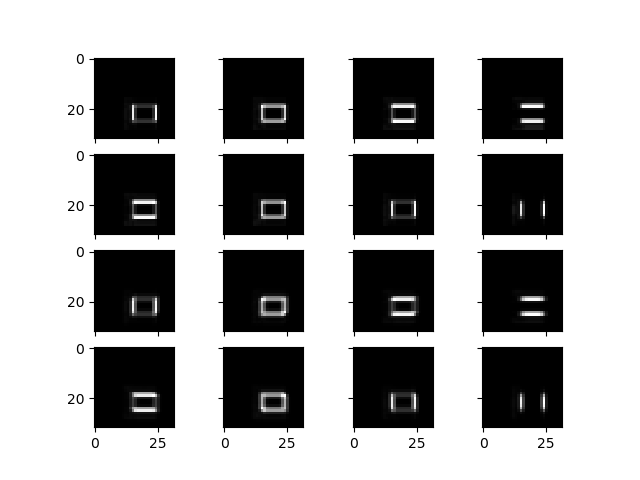
\includegraphics[width=7cm]{images/example2_1ord.png}} &
		\subfloat[]{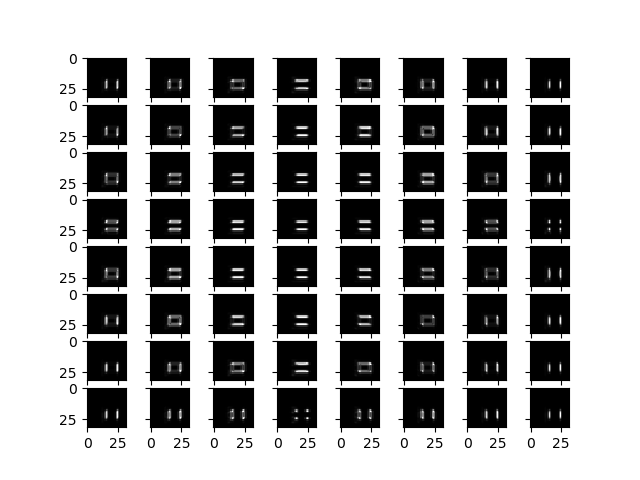
\includegraphics[width=8cm]{images/example2_2ord.png}}
	\end{tabular}
	\caption{Image taken from a toy dataset created for this work. a) Original image; b) 0th order scattering coefficients, i.e. a Gaussian low-pass filter; c) First order scattering coefficients; d) Second order scattering coefficients}
	\label{fig:example2_coefficients}
\end{figure}

%first ellipse
\begin{figure}
	\centering
	\begin{tabular}{cc}
		\subfloat[]{\fbox{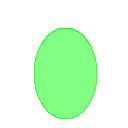
\includegraphics[width=4.5cm]{images/0000027_09.jpg}}} 
		& \subfloat[]{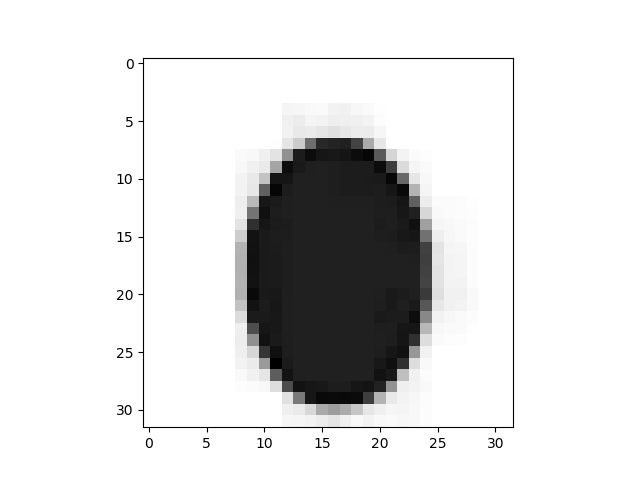
\includegraphics[width=7cm]{images/example1e_0ord.png}}\\
		
		\subfloat[]{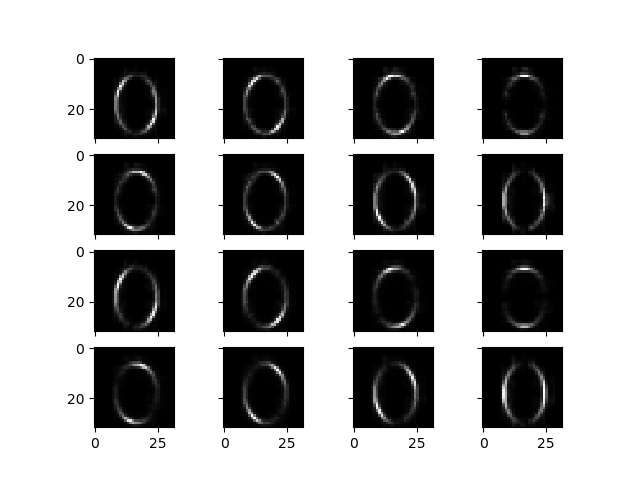
\includegraphics[width=7cm]{images/example1e_1ord.png}} &
		\subfloat[]{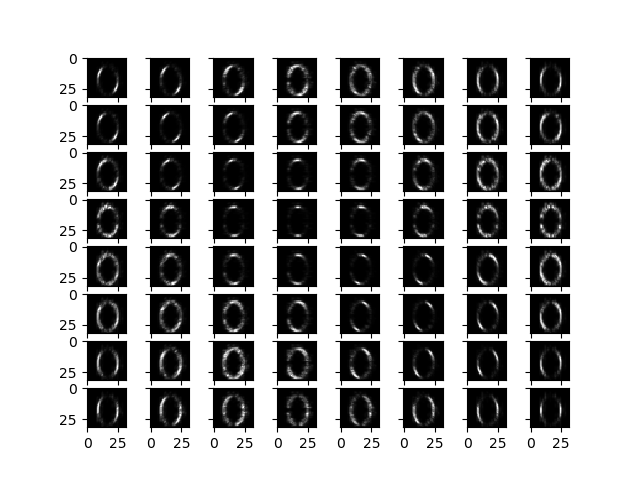
\includegraphics[width=8cm]{images/example1e_2ord.png}}
	\end{tabular}
	\caption{Image taken from a toy dataset created for this work. a) Original image; b) 0th order scattering coefficients, i.e. a Gaussian low-pass filter; c) First order scattering coefficients; d) Second order scattering coefficients}
	\label{fig:example1e_coefficients}
\end{figure}

%second ellipse
\begin{figure}
	\centering
	\begin{tabular}{cc}
		\subfloat[]{\fbox{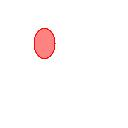
\includegraphics[width=4.5cm]{images/0000027_10.jpg}}} 
		& \subfloat[]{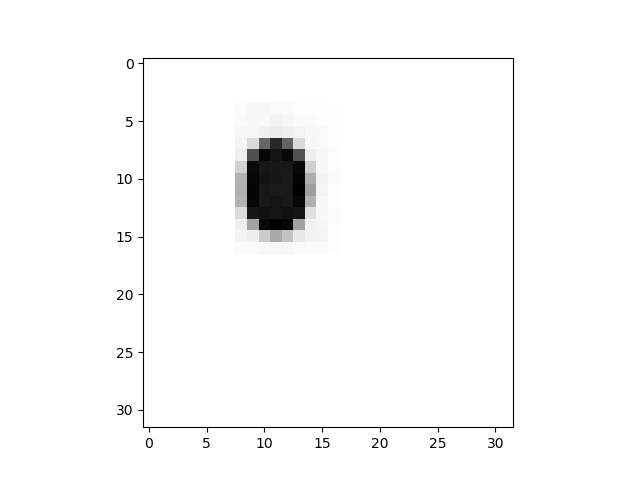
\includegraphics[width=7cm]{images/example2e_0ord.png}}\\
		
		\subfloat[]{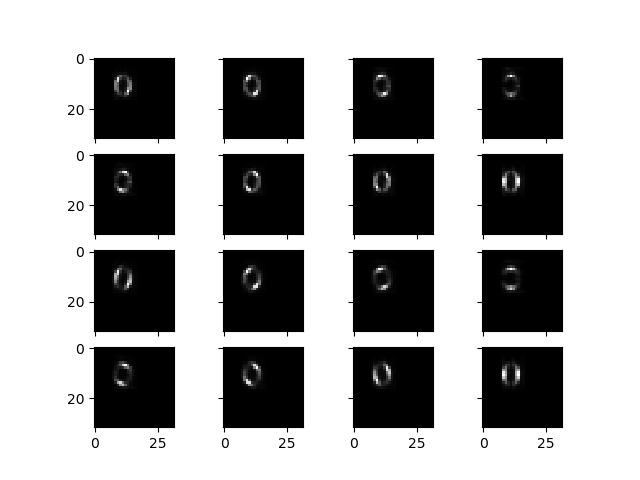
\includegraphics[width=7cm]{images/example2e_1ord.png}} &
		\subfloat[]{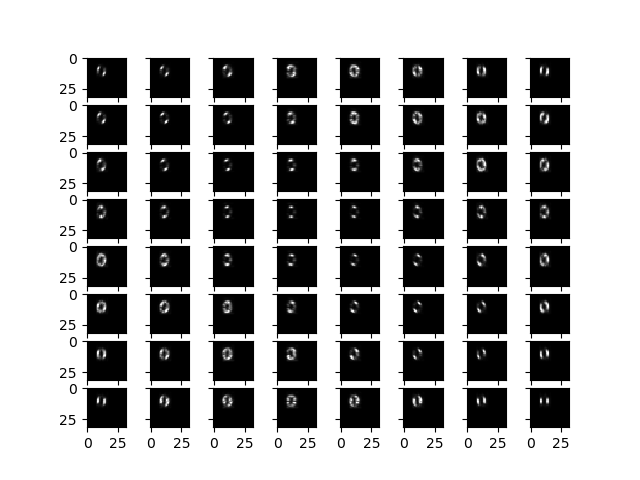
\includegraphics[width=8cm]{images/example2e_2ord.png}}
	\end{tabular}
	\caption{Image taken from a toy dataset created for this work. a) Original image; b) 0th order scattering coefficients, i.e. a Gaussian low-pass filter; c) First order scattering coefficients; d) Second order scattering coefficients}
	\label{fig:example2e_coefficients}
\end{figure}


\section{Results}

\begin{figure}[!htb]
	\centering
%	\begin{tabular}{cccc}
%		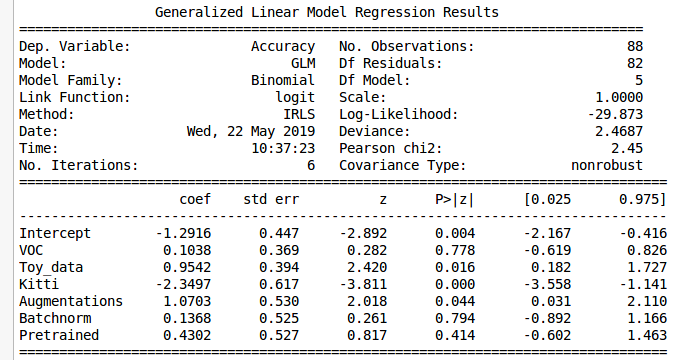
\includegraphics[width=\textwidth]{images/GLM_baselines.png}
%	\end{tabular}
	\begin{center}
		\begin{tabular}{lclc}
			\toprule
			\textbf{Dep. Variable:} &     Accuracy     & \textbf{  No. Observations:  } &       88    \\
			\textbf{Model:}         &       GLM        & \textbf{  Df Residuals:      } &       82    \\
			\textbf{Model Family:}  &     Binomial     & \textbf{  Df Model:          } &        5    \\
			\textbf{Link Function:} &      logit       & \textbf{  Scale:             } &    1.0000   \\
			\textbf{Method:}        &       IRLS       & \textbf{  Log-Likelihood:    } &   -29.873   \\
			\textbf{Date:}          & Wed, 12 Jun 2019 & \textbf{  Deviance:          } &    2.4687   \\
			\textbf{Time:}          &     16:47:27     & \textbf{  Pearson chi2:      } &     2.45    \\
			\bottomrule
		\end{tabular}
		\begin{tabular}{lcccccc}
			& \textbf{coef} & \textbf{std err} & \textbf{z} & \textbf{P$>$$|$z$|$} & \textbf{[0.025} & \textbf{0.975]}  \\
			\midrule
			\textbf{Intercept}     &      -1.2916  &        0.447     &    -2.892  &         0.004        &       -2.167    &       -0.416     \\
			\textbf{VOC}           &       0.1038  &        0.369     &     0.282  &         0.778        &       -0.619    &        0.826     \\
			\textbf{Toy\_data}     &       0.9542  &        0.394     &     2.420  &         0.016        &        0.182    &        1.727     \\
			\textbf{Kitti}         &      -2.3497  &        0.617     &    -3.811  &         0.000        &       -3.558    &       -1.141     \\
			\textbf{Augmentations} &       1.0703  &        0.530     &     2.018  &         0.044        &        0.031    &        2.110     \\
			\textbf{Batchnorm}     &       0.1368  &        0.525     &     0.261  &         0.794        &       -0.892    &        1.166     \\
			\textbf{Pretrained}    &       0.4302  &        0.527     &     0.817  &         0.414        &       -0.602    &        1.463     \\
			\bottomrule
		\end{tabular}
		%\caption{Generalized Linear Model Regression Results}
	\end{center}
	\caption{GLM for the baseline experiments. Positive coefficients imply a better accuracy. P-values below 0.05 are significant.}
	\label{fig:GLM_baseline}
\end{figure}

\begin{figure}[!htb]
	\centering
	\begin{center}
		\begin{tabular}{lclc}
			\toprule
			\textbf{Dep. Variable:}    &     Accuracy     & \textbf{  No. Observations:  } &       42    \\
			\textbf{Model:}            &       GLM        & \textbf{  Df Residuals:      } &       37    \\
			\textbf{Model Family:}     &     Binomial     & \textbf{  Df Model:          } &        4    \\
			\textbf{Link Function:}    &      logit       & \textbf{  Scale:             } &    1.0000   \\
			\textbf{Method:}           &       IRLS       & \textbf{  Log-Likelihood:    } &   -11.790   \\
			\textbf{Date:}             & Wed, 12 Jun 2019 & \textbf{  Deviance:          } &  0.086250   \\
			\textbf{Time:}             &     16:46:44     & \textbf{  Pearson chi2:      } &   0.0930    \\
			\bottomrule
		\end{tabular}
		\begin{tabular}{lcccccc}
			& \textbf{coef} & \textbf{std err} & \textbf{z} & \textbf{P$>$$|$z$|$} & \textbf{[0.025} & \textbf{0.975]}  \\
			\midrule
			\textbf{Intercept}         &      -0.5830  &        1.724     &    -0.338  &         0.735        &       -3.962    &        2.796     \\
			\textbf{Deformation\_data} &       2.9682  &        1.903     &     1.560  &         0.119        &       -0.761    &        6.697     \\
			\textbf{Rotation\_data}    &       1.1550  &        1.756     &     0.658  &         0.511        &       -2.287    &        4.597     \\
			\textbf{Scale\_data}       &       1.2074  &        1.770     &     0.682  &         0.495        &       -2.261    &        4.676     \\
			\textbf{Translation\_data} &      -5.9137  &        6.678     &    -0.886  &         0.376        &      -19.002    &        7.175     \\
			\textbf{Pretrained}        &      -0.0920  &        0.822     &    -0.112  &         0.911        &       -1.704    &        1.520     \\
			\bottomrule
		\end{tabular}
		%\caption{Generalized Linear Model Regression Results}
	\end{center}
	\caption{GLM for the baseline invariant experiments. Positive coefficients imply a better accuracy. P-values below 0.05 are significant.}
	\label{fig:GLM_invariances}
\end{figure}

\begin{figure}[!htb]
	\centering
	\begin{center}
		\begin{tabular}{lclc}
			\toprule
			\textbf{Dep. Variable:}    &     Accuracy     & \textbf{  No. Observations:  } &       40    \\
			\textbf{Model:}            &       GLM        & \textbf{  Df Residuals:      } &       32    \\
			\textbf{Model Family:}     &     Binomial     & \textbf{  Df Model:          } &        7    \\
			\textbf{Link Function:}    &      logit       & \textbf{  Scale:             } &    1.0000   \\
			\textbf{Method:}           &       IRLS       & \textbf{  Log-Likelihood:    } &   -13.468   \\
			\textbf{Date:}             & Fri, 14 Jun 2019 & \textbf{  Deviance:          } &   0.45398   \\
			\textbf{Time:}             &     16:16:06     & \textbf{  Pearson chi2:      } &    0.504    \\
			\bottomrule
		\end{tabular}
		\begin{tabular}{lcccccc}
			& \textbf{coef} & \textbf{std err} & \textbf{z} & \textbf{P$>$$|$z$|$} & \textbf{[0.025} & \textbf{0.975]}  \\
			\midrule
			\textbf{Intercept}         &       0.5339  &        0.515     &     1.037  &         0.300        &       -0.475    &        1.543     \\
			\textbf{VOC}               &      -0.8504  &        0.959     &    -0.887  &         0.375        &       -2.729    &        1.029     \\
			\textbf{Kitti}             &      -2.7801  &        1.273     &    -2.184  &         0.029        &       -5.275    &       -0.285     \\
			\textbf{Toy\_data}         &       1.0364  &        1.005     &     1.031  &         0.303        &       -0.934    &        3.007     \\
			\textbf{Deformation\_data} &       2.0923  &        1.446     &     1.447  &         0.148        &       -0.742    &        4.927     \\
			\textbf{Rotation\_data}    &       0.0003  &        0.825     &     0.000  &         1.000        &       -1.616    &        1.617     \\
			\textbf{Scale\_data}       &       0.0821  &        0.832     &     0.099  &         0.921        &       -1.549    &        1.713     \\
			\textbf{Translation\_data} &       0.9533  &        0.983     &     0.970  &         0.332        &       -0.973    &        2.880     \\
			\textbf{Pretrained}        &      -0.0502  &        0.789     &    -0.064  &         0.949        &       -1.596    &        1.495     \\
			\bottomrule
		\end{tabular}
		%\caption{Generalized Linear Model Regression Results}
	\end{center}
\caption{GLM for the sequential scattering experiments. Positive coefficients imply a better accuracy. P-values below 0.05 are significant.}
\label{fig:GLM_sequential_scattering}
\end{figure}

\begin{figure}[!htb]
	\centering
	\begin{center}
		\begin{tabular}{lclc}
			\toprule
			\textbf{Dep. Variable:}    &     Accuracy     & \textbf{  No. Observations:  } &       23    \\
			\textbf{Model:}            &       GLM        & \textbf{  Df Residuals:      } &       15    \\
			\textbf{Model Family:}     &     Binomial     & \textbf{  Df Model:          } &        7    \\
			\textbf{Link Function:}    &      logit       & \textbf{  Scale:             } &    1.0000   \\
			\textbf{Method:}           &       IRLS       & \textbf{  Log-Likelihood:    } &   -8.0343   \\
			\textbf{Date:}             & Mon, 17 Jun 2019 & \textbf{  Deviance:          } &   0.30082   \\
			\textbf{Time:}             &     18:08:03     & \textbf{  Pearson chi2:      } &    0.291    \\
			\bottomrule
		\end{tabular}
		\begin{tabular}{lcccccc}
			& \textbf{coef} & \textbf{std err} & \textbf{z} & \textbf{P$>$$|$z$|$} & \textbf{[0.025} & \textbf{0.975]}  \\
			\midrule
			\textbf{Intercept}         &       0.2852  &        0.715     &     0.399  &         0.690        &       -1.116    &        1.686     \\
			\textbf{VOC}               &      -1.1895  &        1.435     &    -0.829  &         0.407        &       -4.003    &        1.624     \\
			\textbf{Kitti}             &      -2.9350  &        2.418     &    -1.214  &         0.225        &       -7.674    &        1.803     \\
			\textbf{Toy\_data}         &       0.8272  &        1.169     &     0.708  &         0.479        &       -1.463    &        3.118     \\
			\textbf{Deformation\_data} &       1.8665  &        1.824     &     1.023  &         0.306        &       -1.708    &        5.441     \\
			\textbf{Rotation\_data}    &       0.2194  &        1.061     &     0.207  &         0.836        &       -1.860    &        2.299     \\
			\textbf{Scale\_data}       &       0.1882  &        1.057     &     0.178  &         0.859        &       -1.884    &        2.261     \\
			\textbf{Translation\_data} &       1.3084  &        1.317     &     0.994  &         0.320        &       -1.272    &        3.889     \\
			\textbf{Pretrained}        &       0.2116  &        1.020     &     0.207  &         0.836        &       -1.787    &        2.211     \\
			\bottomrule
		\end{tabular}
		%\caption{Generalized Linear Model Regression Results}
	\end{center}
\caption{GLM for the parallel scattering experiments. Positive coefficients imply a better accuracy. P-values below 0.05 are significant.}
\label{fig:GLM_parallel_scattering}
\end{figure}

\begin{figure}[!htb]
	\centering
	\begin{center}
		\begin{tabular}{lclc}
			\toprule
			\textbf{Dep. Variable:}         &     Accuracy     & \textbf{  No. Observations:  } &       36    \\
			\textbf{Model:}                 &       GLM        & \textbf{  Df Residuals:      } &       31    \\
			\textbf{Model Family:}          &     Binomial     & \textbf{  Df Model:          } &        4    \\
			\textbf{Link Function:}         &      logit       & \textbf{  Scale:             } &    1.0000   \\
			\textbf{Method:}                &       IRLS       & \textbf{  Log-Likelihood:    } &   -8.0310   \\
			\textbf{Date:}                  & Wed, 12 Jun 2019 & \textbf{  Deviance:          } &    1.3209   \\
			\textbf{Time:}                  &     16:43:30     & \textbf{  Pearson chi2:      } &     1.27    \\
			\bottomrule
		\end{tabular}
		\begin{tabular}{lcccccc}
			& \textbf{coef} & \textbf{std err} & \textbf{z} & \textbf{P$>$$|$z$|$} & \textbf{[0.025} & \textbf{0.975]}  \\
			\midrule
			\textbf{Intercept}              &      -1.0483  &        0.356     &    -2.947  &         0.003        &       -1.745    &       -0.351     \\
			\textbf{Toy\_data\_small}       &       0.6860  &        0.549     &     1.250  &         0.211        &       -0.390    &        1.762     \\
			\textbf{VOC}                    &      -1.7343  &        0.706     &    -2.457  &         0.014        &       -3.118    &       -0.351     \\
			\textbf{twentyfivek}            &       1.1156  &        0.637     &     1.751  &         0.080        &       -0.133    &        2.364     \\
			\textbf{fivek}                  &      -2.1638  &        0.881     &    -2.457  &         0.014        &       -3.890    &       -0.437     \\
			\textbf{standard}               &       0.2188  &        0.735     &     0.298  &         0.766        &       -1.222    &        1.660     \\
			\textbf{sequential\_scattering} &       0.0583  &        0.740     &     0.079  &         0.937        &       -1.392    &        1.509     \\
			\textbf{parallel\_scattering}   &      -1.3253  &        0.887     &    -1.494  &         0.135        &       -3.064    &        0.413     \\
			\bottomrule
		\end{tabular}
		%\caption{Generalized Linear Model Regression Results}
	\end{center}
	\caption{GLM for the small data experiments. Positive coefficients imply a better accuracy. P-values below 0.05 are significant.}
	\label{fig:GLM_small_data}
\end{figure}
